\documentclass{article}
\title{Controle de máquina motora monofásica}
\date{}

\usepackage[utf8]{inputenc}
\usepackage[portuguese]{babel}
\usepackage[margin=2.5cm]{geometry}
\usepackage{amsmath}
\usepackage{physics}
\usepackage{pgfplots}
\pgfplotsset{compat = newest}
\usepackage{titlesec}
\usepackage{graphicx}
\usepackage{wrapfig}
\usepackage{caption}
\usepackage{subcaption}
\usepackage{tabularx}
\usepackage[parfill]{parskip}
\usepackage[nottoc]{tocbibind}
\usepackage[backend=biber]{biblatex}
\addbibresource{/home/luispengler/drive/LinuxFabrik/Research/read/bib.bib}
\usepackage{authblk}
\renewcommand\Authand{ e }
\renewcommand\Authands{ e }
\author[1]{Luís Spengler}
\author[2]{Raquel Braiani}
\affil[1,2]{Instituto Federal de Educação, Ciência e Tecnologia de Mato Grosso do Sul}

\begin{document}
\maketitle

\section{Introdução}
Adentrando na parte de controle, fomos instruidos a montagem de um circuito contendo um motor monofásico. O controle realizado no motor, embora simples, cria uma base para um posterior aprofundamento da disciplina.

\section{Problemática}
O controle efetuado justifica-se na necessidade de ter uma máquina motor operando em apenas uma área delimitada e que uma vez ao fim do percurso, tendo realizado sua função, esta desliga-se.

\section{Objetivo Geral}
\begin{itemize}
	\item Identificar, esquematizar e montar um circuito de controle
\end{itemize}

\section{Metodologia}
Para identificação e esquematização do circuito, o professor Msc. Hilton James apresentou-nos um aplicativo chamado ``simurelay'', onde é possível esquematizar e simular diversos circuitos de máquinas elétricas.

\begin{figure}[h!]
	\centering
        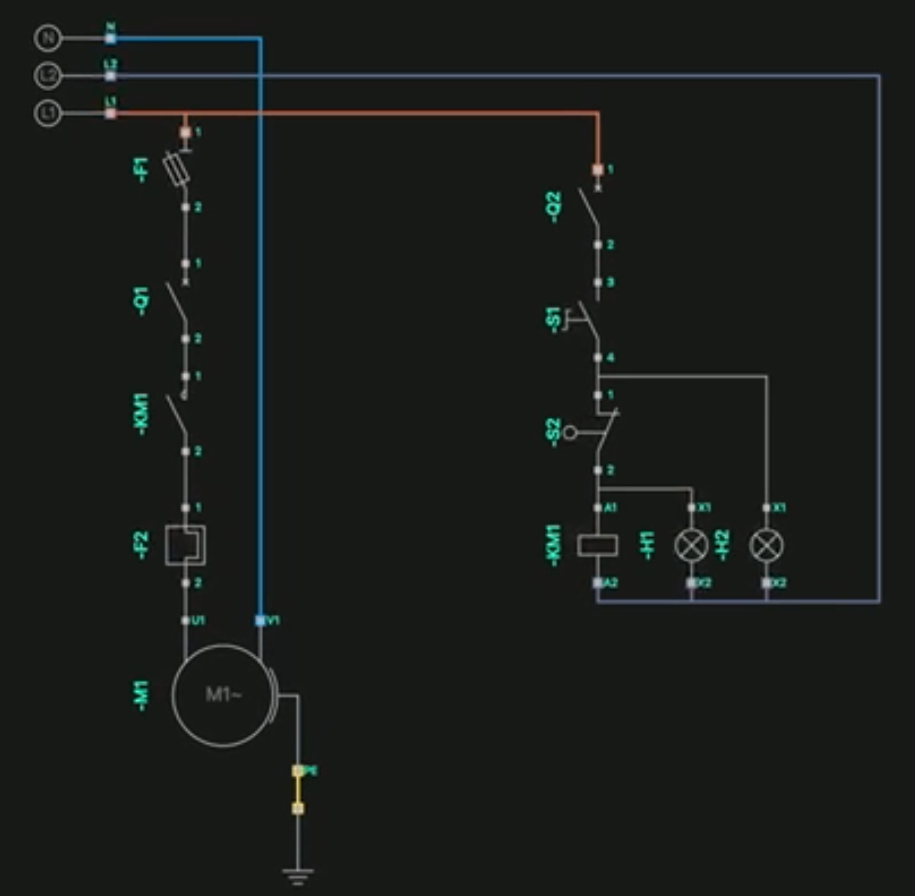
\includegraphics[width=0.45\textwidth]{simurelay}
	\caption{Esquema do circuito desligado no simurelay, pois a chave que liga o sistema está aberta}
\end{figure}

A parte de controle conta com uma chave fim de curso normalmente fechada, ou seja, o circuito estará sempre ligado se a chave fim de curso não for acionada. No caso prático, a chave é acionada quando a variável controlada (posição) está em um determinado ponto (setpoint) e então a chave fim de curso NF abre, esta sempre atuando na corrente elétrica (variavél manipulada).

\begin{figure}[h!]
	\centering
        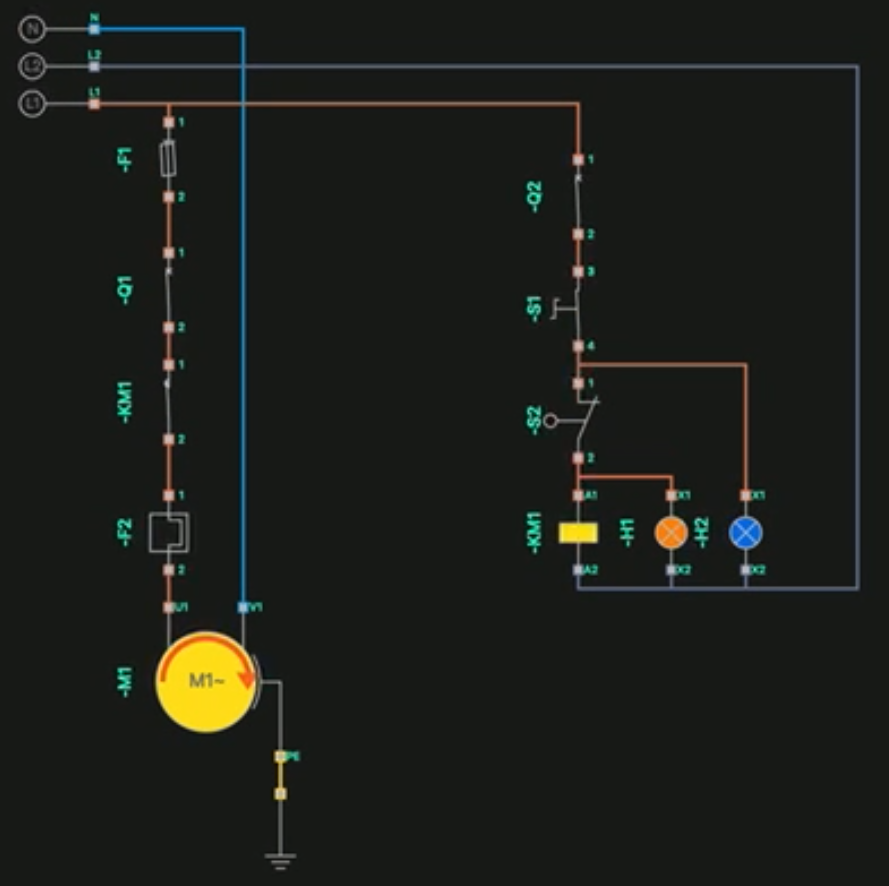
\includegraphics[width=0.45\textwidth]{simurelay1}
	\caption{Esquema do circuito ligado no simurelay, pois a chave que liga o sistema está fechada e a chave fim de curso não foi acionada}
\end{figure}

\section{Resultados}
Pode-se identificar o tipo de controle como sendo liga-desliga, pois a única ação que acontece é ligar ou desligar o controle de acordo com a atuação da chave fim de curso.

\section{Conclusão}
Foi possivel identificar, esquematizar e montar um circuito de controle que fizesse com que uma máquina motor operasse ou não dependendo do estado de uma chave fim de curso.

\end{document}
